\documentclass[letter]{article}
\renewcommand{\baselinestretch}{1.25}

\usepackage[margin=1in]{geometry}
\usepackage{physics}
\usepackage{amsmath}
\usepackage{amssymb}
\usepackage{graphicx}
\usepackage{hyperref}

% MATLAB Formating Code
\usepackage[numbered,framed]{matlab-prettifier}
\lstset{style=Matlab-editor,columns=fullflexible}
\renewcommand{\lstlistingname}{Script}
\newcommand{\scriptname}{\lstlistingname}

% Document Specific
\newcommand{\sat}{\text{sat}}

\allowdisplaybreaks

%opening
\title{MECH 6313 - Homework 6}
\author{Jonas Wagner}
\date{2021, April 28}

\begin{document}

\maketitle

\tableofcontents

\newpage
\section{Problem 1}
\textbf{Problem:}
Show that the parallel connection of two passive dynamical systems is passive. Can you claim the same for the series connection of two passive systems?

\textbf{Solution:}
Let two passive systems be defined as a system taking an input $u$ and generating an output $y$ as $$H_1: y_1= h_1(u), \ \text{s.t.} \ \braket{y_1}{u} \geq 0$$ and $$H_2: y_2 = h_2(u), \ \text{s.t.} \ \braket{y_2}{u} \geq 0$$
with $\braket{y}{u} = \int_0^T y^T(t) u(t) \dd{t}$

\subsection{Parallel Connection of Passive System}
The parallel system $H_p$ can then be defined by $$H_p : h_p(u) = y_p = y_1 + y_2 = h_1(u) + h_2(u)$$ whose passivity can be proven directly by testing $\braket{y_p}{u}$ which is calculated as
\begin{align}
	\braket{y_p}{u} &= \int_0^T y_p^T u \dd{t}\\
	&= \int_0^T (y_1 + y_2)^T u \dd{t}\\
	&= \int_0^T y_1^T u + y_2^T u \dd{t}\\
	&= \int_0^T y_1^T u \dd{t} + \int_0^T y_2^T u \dd{t}\\
	&= \braket{y_1}{u} + \braket{y_2}{u}
	\intertext{Since $ \braket{y_1}{u} \geq 0$ and $\braket{y_2}{u} \geq 0$,}
	\braket{y_p}{u} &\geq 0
\end{align}
which proves, by definition, that $H_p$ is passive.

\newpage
\subsection{Series Connection of Passive System}
The series system $H_s$ can be defined by $$H_s : h_s(u) = y_s = h_1(u) \circledast h_2(u)  = h_2(h_1(u))$$
whose passivity can be tested using $\braket{y_s}{u}$ which is calculated as:
\begin{align}
	\braket{y_s}{u} &= \int_0^T y_s^T u \dd{t}\\
	&= \int_0^T \qty(h_1 (u) \circledast h_2(u))^T u \dd{t}\\
	&= \int_0^T \qty(\int_0^T h_1(t - \tau) h_2(\tau) \dd{\tau}) \dd{t}\\
	&= \int_0^T h_2(\tau) \qty(\int_0^T h_1(t - \tau)  \dd{t}) \dd{\tau}
\end{align}
which is not explicitly $\geq 0$ so this method cannot prove passivity.

A different method of analysis can be done to prove that this is not passive in general, but a counter example from MATLAB (\appendixname \ \ref{apx:matlab}) can be shown to not be passive due to a loss of positive realness of the transfer functions when placed in series:
$$G_1(s) = \cfrac{5s^2 + 3s + 1}{s^2 + 2s + 1}, \ G_2(s) = \cfrac{s^3 + s^2 + 5s + 0.1}{s^3 + 2s^2 + 3s + 4}$$
and when combined in series the system is no longer passive due to a loss of positive realness.
$$ \cfrac{5 s^5 + 8 s^4 + 29 s^3 + 16.5 s^2 + 5.3 s + 0.1}{s^5 + 4 s^4 + 8 s^3 + 12 s^2 + 11 s + 4}$$

\newpage
\section{Problem 2}
Let $$H(s) = \cfrac{s+\lambda}{s^2 + a s + b}$$ with $a>0$ and $b>0$.

\subsection{Part a}
\textbf{Problem:}
For which values of $\lambda$ is $H(s)$ Positive Real (PR)?\\

\noindent
\textbf{Solution:}
By definition, a transfer function must satisfy two conditions to be considered Postive Real:
\begin{enumerate}
	\item $\real\{\lambda(H(s))\} \leq 0$, any $j\omega$ roots are simple, and any residuals are non negative.
	\item $\real\{H(j\omega)\} \geq 0 \ \forall \omega \in \real$
\end{enumerate}

The transfer function for this problem will always satisfy the first condition, however, the second condition is violated under the following conditions:\\

Setting $$s = j\omega$$
\begin{align}
	H(j\omega) &= \cfrac{j\omega + \lambda}{(j\omega)^2 + a (j\omega) + b}
	= \cfrac{j\omega + \lambda}{-\omega^2 + j a \omega + b}\\
	&= \cfrac{-\omega^2 - j a \omega + b}{-\omega^2 - j a \omega + b} \cdot \cfrac{j\omega + \lambda}{-\omega^2 + j a \omega + b}\\
	&= \cfrac{\qty(a \omega^2 + \lambda (\omega^2 + b)) + j \qty(\omega (\omega^2 + b) - a \lambda \omega)}{a^2 \omega^2 + (\omega^2 + b)^2}\\
	&= \cfrac{a \omega^2 + \lambda (\omega^2 + b)}{a^2 \omega^2 + (\omega^2 + b)^2} + j \cfrac{\omega (\omega^2 + b) - a \lambda \omega}{a^2 \omega^2 + (\omega^2 + b)^2}
\end{align}

The real component being nonnegative can then be seen to occur when
\begin{align}
	a \omega^2 + \lambda (\omega^2 + b) \geq 0\\
	\lambda (\omega^2 + b) \geq -a \omega^2\\
	\lambda \geq \cfrac{-a\omega^2}{\omega^2 + b}
\end{align}

Since this mus apply $\forall \omega \in \real$, the following must be true
\begin{align}
	\lambda \geq 0
\end{align}

\newpage
\subsection{Part b}
\textbf{Problem:}
Using the results from above, select $\lambda_1, \lambda_2$ such that
\begin{align}
	H_1(s) &= \cfrac{s+\lambda_1}{s^2 + s + 1} \text{ is PR}\\
	H_2(s) &= \cfrac{s+\lambda_2}{s^2 + s + 1} \text{ is not PR}
\end{align}
Then verify the PR properties for each using the Nyquist plots of $H_1(s)$ and $H_2(s)$.\\

\noindent
\textbf{Solution:}
From the requirements set above, the zeros can be selected with $\lambda_1 = 1$ and $\lambda_2 = -1$ resulting in $H_1(s)$ and $H_2(s)$ being defined as
\begin{align}
	H_1(s) &= \cfrac{s+1}{s^2 + s + 1}\\
	H_2(s) &= \cfrac{s-1}{s^2 + s + 1}
\end{align}

The nyquist plots, generated with the MATLAB code seen in \appendixname \ \ref{apx:matlab}, can then be used to verify the PR properties. As can be seen in \figurename \ \ref{fig:pblm2h1}, the nyquist diagram for $H_1(s)$ never crosses into the LHP and therefore is Positive Real. Conversely, in \figurename \ \ref{fig:pblm2h2}, the nyquist diagram for $H_2(s)$ crosses into the LHP and therefore is not Positive Real.

\begin{figure}[p]
	\centering
	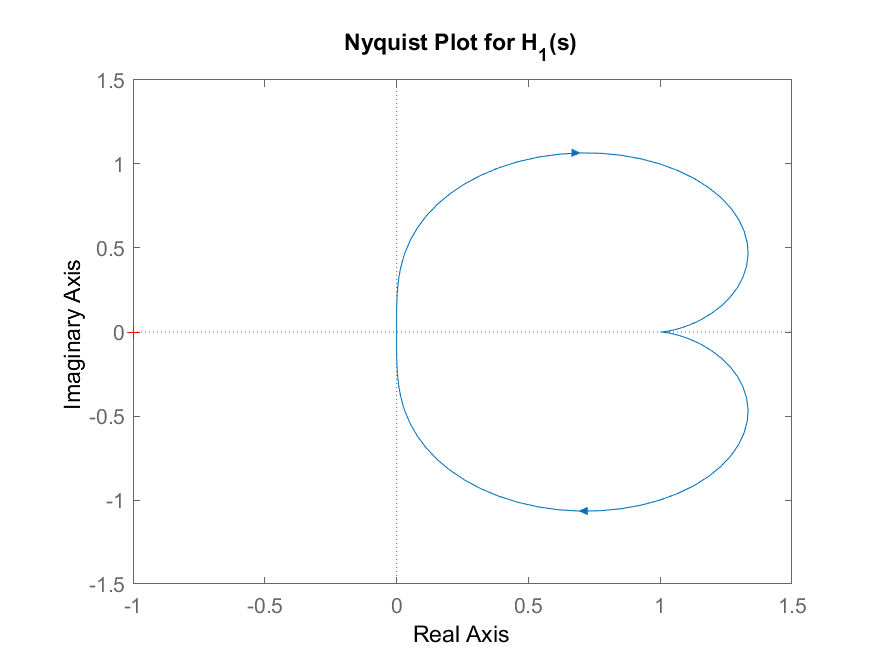
\includegraphics[width=0.7\linewidth]{fig/pblm2_H1}
	\caption{Nyquist Plot for the $H_1(s)$ transfer function.}
	\label{fig:pblm2h1}
\end{figure}

\begin{figure}[p]
	\centering
	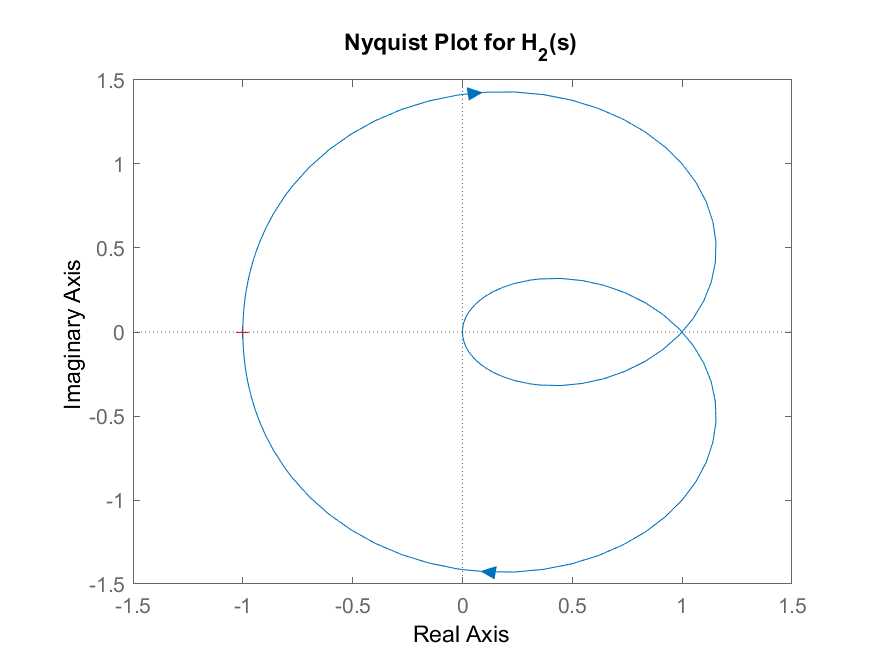
\includegraphics[width=0.7\linewidth]{fig/pblm2_H2}
	\caption{Nyquist Plot for the $H_2(s)$ transfer function.}
	\label{fig:pblm2h2}
\end{figure}

\newpage
\subsection{Part c}
\textbf{Problem:}
For $H_1(s)$ and $H_2(s)$, write state-space realizations and solve for $P=P^T > 0$ in the PR lemma and explain why it fails for $H_2(s)$.\\

\noindent
\textbf{Solution:}
Given a second order transfer function $$\cfrac{s + b_0}{s^2 + a_1 s + a_0}$$ a state space system can be defined by:
\begin{equation}
	\begin{aligned}
		&A = \mqty[0 &1\\ -a_0 &-a_1] \hspace{0.5in} &&B = \mqty[0\\ 1]\\
		&C = \mqty[b_0 & 1] \hspace{0.5in} &&D = 0
	\end{aligned}
\end{equation}

This can be applied to the systems and results in the state space representations of $H_1$ as:
\begin{equation}\label{eq:H_1}
	\begin{aligned}
		&A = \mqty[0 &1\\ -1 &-1] \hspace{0.5in} &&B = \mqty[0\\ 1]\\
		&C = \mqty[1 & 1] \hspace{0.5in} &&D = 0
	\end{aligned}
\end{equation}
and $H_2$ as
\begin{equation}\label{eq:H_2}
	\begin{aligned}
		&A = \mqty[0 &1\\ -1 &-1] \hspace{0.5in} &&B = \mqty[0\\ 1]\\
		&C = \mqty[-1 & 1] \hspace{0.5in} &&D = 0
	\end{aligned}
\end{equation}

Each of these systems can be tested for passivity by solving for a $P=P^T>0$ s.t.
\begin{align}
	A^T P + P A < 0\\
	PB = C^T
\end{align}

Additionally, let $$P = \mqty[p_{11} & p_{12}\\ p_{12} & p_{22}]$$

\newpage
%H_1 --------------------------------------------------------
$H_1(s)$ was found in \eqref{eq:H_1}to be
\begin{equation}\nonumber
	\begin{aligned}
		&A = \mqty[0 &1\\ -1 &-1] \hspace{0.5in} &&B = \mqty[0\\ 1]\\
		&C = \mqty[1 & 1] \hspace{0.5in} &&D = 0
	\end{aligned}
\end{equation}
and can be proven to be passive by solving the following LMI:
\begin{align}
	A^T P + P A &\leq 0\\
	P B - C^T &= 0
\end{align}
\begin{align}
	\mqty[0 &1\\ -1 &-1]^T \mqty[p_{11} & p_{12}\\ p_{12} & p_{22}] + \mqty[p_{11} & p_{12}\\ p_{12} & p_{22}] \mqty[0 &1\\ -1 &-1] &\leq 0\\
	\mqty[p_{11} & p_{12}\\ p_{12} & p_{22}] \mqty[0\\ 1] - \mqty[1 & 1]^T &= 0
\end{align}

\begin{align}
	\mqty[-2p_{12} & p_{11} - p_{12} - p_{22}\\ p_{11} - p_{12} - p_{22} & 2 p_{12} - 2 p_{22}] &\leq 0\\
	p_{12} - 1 &= 0\\
	p_{22} - 1 &= 0
\end{align}
Two coefficients can then clearly be defined resulting in
\begin{align}
	p_{12} &= 1\\
	p_{22} &= 1\\
	\mqty[-2(1) & p_{11} - (1) - (1)\\ p_{11} - (1) - (1) & 2 (1) - 2 (1)] &\leq 0
\end{align}

\begin{align}
	\mqty[-2 & p_{11} - 2\\ p_{11} - 2 & 0] \leq 0
\end{align}

Which is equivalent to the standard PSD equation: 
\begin{align}
	\mqty[2 & 2 - p_{11}\\ 2 - p_{11} & 0] \geq 0
\end{align}

And to ensure this is PSD, the principle minors can be analyzed:
\begin{align}
	a = 2 &> 0\\
	\det\mqty[2 & 2 - p_{11}\\ 2 - p_{11} & 0] &\geq 0\\
	-(2-p_{11})(2-p_{11}) &\geq 0\\
	-4 +2 p_{11} - p_{11}^2 &\geq 0
\end{align}
it is clear that a solution of $p_{11} = 0$ results in a PSD matrix and thus a Positive Real and passive system.

\newpage
% H_2 -----------------------------------------------------------
$H_2(s)$ was found in \eqref{eq:H_2} to be
\begin{equation}\nonumber
	\begin{aligned}
		&A = \mqty[0 &1\\ -1 &-1] \hspace{0.5in} &&B = \mqty[0\\ 1]\\
		&C = \mqty[-1 & 1] \hspace{0.5in} &&D = 0
	\end{aligned}
\end{equation}
and can be proven to be passive by solving the following LMI
\begin{align}
	A^T P + P A &\leq 0\\
	P B - C^T &= 0
\end{align}

\begin{align}
	\mqty[0 &1\\ -1 &-1]^T \mqty[p_{11} & p_{12}\\ p_{12} & p_{22}] + \mqty[p_{11} & p_{12}\\ p_{12} & p_{22}] \mqty[0 &1\\ -1 &-1] &\leq 0\\
	\mqty[p_{11} & p_{12}\\ p_{12} & p_{22}] \mqty[0\\ 1] - \mqty[-1 & 1]^T &= 0
\end{align}

\begin{align}
	\mqty[-2p_{12} & p_{11} - p_{12} - p_{22}\\ p_{11} - p_{12} - p_{22} & 2 p_{12} - 2 p_{22}] &\leq 0\\
	p_{12} + 1 &= 0\\
	p_{22} - 1 &= 0
\end{align}

Two coefficients can then clearly be defined resulting in
\begin{align}
	p_{12} &= -1\\
	p_{22} &= 1\\
	\mqty[-2(-1) & p_{11} - (-1) - (1)\\ p_{11} - (-1) - (1) & 2 (-1) - 2 (1)] &\leq 0
\end{align}

\begin{align}
	\mqty[2 & p_{11}\\ p_{11}& -4] \leq 0
\end{align}

Which is equivalent to the standard PSD equation:
\begin{align}
	\mqty[-2 & -p_{11}\\ -p_{11}& 4] \geq 0
\end{align}

And this is clearly not capable of being PSD due to the first principle minor being negative. Therefore, the system is not Positive Real and cannot be passive.

\newpage
\section{Problem 3}
Consider the following 3-stage ring oscillator discussed in class:
\begin{align*}
	\tau_1 \dot{x}_1 &= -x_1 - \alpha_1 \tanh(\beta_1 x_3)\\
	\tau_2 \dot{x}_2 &= -x_2 - \alpha_2 \tanh(\beta_2 x_1)\\
	\tau_3 \dot{x}_3 &= -x_3 - \alpha_3 \tanh(\beta_3 x_2)
\end{align*}
with $\tau_i, \alpha_i, \beta_i > 0$ and $x_i$ represents a voltage for $i = 1,2,3$.

\subsection{Part a}
\textbf{Problem:}
Suppose $\alpha_1 \beta_1 = \alpha_2 \beta_2 = \alpha_3 \beta_3 = \mu$, prove the origin is GAS when $\mu < 2$.\\

\noindent
\textbf{Solution:}
The 3-stage ring oscillator can be rewritten in a coupling feedback system $H$ and $K$ defined as:
\begin{align}
	H &= \mqty[\dmat{H_1}{H_2}{H_3}], \hspace{0.25in}
	H_i
	=\begin{cases}
		\dot{x}_i = f(x_i) + g(x_i) u_i\\
		y_i = h(x_i)
	\end{cases}\\
	K &= \mqty[	 0 	& 0 &-1\\
				-1 	& 0 & 0\\
				0 	&-1 & 0]
\end{align}
where $K$ is the coupling matrix of the individual nonlinear subsystems with the following specific definitions:
\begin{align}
	H_i &=\begin{cases}
		\dot{x}_i = \cfrac{-x_i + u_i}{\tau_i}\\
		y_i = \alpha_j \tanh(\beta_j x_i)
	\end{cases}\\
	\intertext{with $j$ being defined as either $i+1$ or $1$ if $i=n$, resulting in}
	H_1 &=\begin{cases}
		\dot{x}_1 = \cfrac{-x_1 + u_1}{\tau_1}\\
		y_1 = \alpha_2 \tanh(\beta_2 x_1)
	\end{cases}\\
	H_2 &=\begin{cases}
		\dot{x}_2 = \cfrac{-x_2 + u_2}{\tau_2}\\
		y_2 = \alpha_3 \tanh(\beta_3 x_2)
	\end{cases}\\
	H_3 &=\begin{cases}
		\dot{x}_3 = \cfrac{-x_3 + u_3}{\tau_3}\\
		y_3 = \alpha_1 \tanh(\beta_1 x_3)
	\end{cases}
\end{align}

\newpage
From this model a storage function can be defined for each of the coupled systems as
\begin{align}
	V_i(x_i) &= \tau_i \int_0^{x_i} h_i(\eta) \dd{\eta}\\
	\intertext{and each individual subsystem storage functions are given as:}
	V_1(x_1) &= \tau_1 \int_0^{x_1} \alpha_2 \tanh(\beta_2 x_1)\\
	V_2(x_2) &= \tau_2 \int_0^{x_2} \alpha_3 \tanh(\beta_3 x_2)\\
	V_3(x_3) &= \tau_3 \int_0^{x_3} \alpha_1 \tanh(\beta_1 x_3)
\end{align}

Taking a look at the change of the storage function over time, the output strict passivity can be proven by:
\begin{align}
	\dot{V}_i (x_i) &= \dv{V_i}{x_i} \dot{x}_i\\
	&= \dv{x_i} \tau_i \int_0^{x_i} h_i(\eta) \dd{\eta} \dot{x}_i\\
	&= \tau_i h_i(x_i) \dot{x}_i
	\intertext{taking the definition for $\dot{x}_i$ and relating $h_i(x_i) = y_i$,}
	&= \tau_i h_i(x_i) \frac{-x_i + u_i}{\tau_i}\\
	&= -x_i h_i(x_i) + u_i y_i
\end{align}

\newpage
In order to guarantee Input passivity, the system must satisfy the following inequality:
\begin{align}
	x h(x) &\leq \delta_i x^2\\
	x (\alpha \tanh(\beta x)) &\leq \delta x^2
\end{align}
by definition, $\alpha, \beta > 0$ and $\delta \geq 0$, and thus the following inequalities apply:
\begin{align}
	\begin{cases}
		\alpha \tanh(\beta x) > 0, &x>0\\
		\alpha \tanh(\beta x) < 0, &x<0
	\end{cases}
\end{align}
therefore, when $$\abs{\alpha \tanh(\beta x)} \leq \abs{\delta x}$$ the input passivity equality holds.
This occurs whenever $$\alpha \beta = \mu \leq \delta$$, so $\delta$ is the limiting factor that is restricted by the storage function calculation.\\

In the case that input passivity is satisfied by $h_i(x_i)$, a $\delta_i$ will exist s.t.,
\begin{align}
	x_i h_i(x_i) &\leq \delta_i x^2\\
	x_i (h_i(x_i) - \delta_i x_i) &\leq 0
\end{align}
clearly, $x_i h_i(x_i)$ can then be bounded from below by: % since \abs{h_i} \leq \abs{\delta_i x} \forall x
\begin{align}
	x_i h_i (x) \geq \frac{1}{\delta_i} h_i^2(x_i)\\
	-x_i h_i (x) \geq -\frac{1}{\delta_i} h_i^2(x_i)\\
	\intertext{since $y_i = h_i(x_i)$,}
	-x_i h_i (x) \geq -\frac{1}{\delta_i} y_i^2(x_i)
\end{align}

%\newpage
Therefore, this demonstrates Output Strict Passivity:
\begin{align}
	\dot{V}_i &\leq -\frac{1}{\delta_i} y_i^2 + y_i u_i\\
	\intertext{or with $d_i = \frac{1}{\delta_i}$ and }
	\dot{V}_i &\leq d_i y_i^2 + y_i u_i
\end{align}
and the passivity theorem can then be applied.

Let $$\epsilon_i = \frac{1}{\delta_i} \leq \frac{1}{\mu}$$ and then define
\begin{align}
	A &= - \text{diag}\{\epsilon_i\} + K\\
	P &= \text{diag}\{d_i\}
\end{align}
which for this $3^{rd}$-order system can be written as
\begin{align}
	A &= -\mqty[\dmat{\epsilon_1}{\epsilon_2}{\epsilon_3}] + \mqty[0 & 0 &-1\\ -1 & 0 & 0\\ 0 &-1 & 0] 
	= \mqty[-\epsilon_1 & 0 &-1\\
			 -1 &-\epsilon_2 &0\\
			 0	&-1	&-\epsilon_3]\\
	P &= \mqty[\dmat{d_1}{d_2}{d_3}]
\end{align}

From this, appropriate values for A and P can be found using CVX to prove stability of the full feedback interconnection by solving the feasibility problem of
\begin{align}
	A^T P + P A &\leq 0
\end{align}
with $C$ defined as the output matrix associated with the actual state-space representation.

This can then be further developed to prove Global Asymptotic Stability by making it a strict inequality like so:
\begin{align}
	A^T P + P A &< 0
\end{align}
Which can be expanded with the actual matrices as
\begin{align}
	\mqty[-\epsilon_1 & 0 &-1\\
	-1 &-\epsilon_2 &0\\
	0	&-1	&-\epsilon_3]^T
	\mqty[\dmat{d_1}{d_2}{d_3}] +
	\mqty[\dmat{d_1}{d_2}{d_3}]
	\mqty[-\epsilon_1 & 0 &-1\\
	-1 &-\epsilon_2 &0\\
	0	&-1	&-\epsilon_3]
	&< 0
\end{align}

\begin{align}
	\mqty[-d_1\epsilon_1 & -d_1 &0\\
		0 &-d_2\epsilon_2 &-d_2\\
		-d_3	&0	&-d_3\epsilon_3]+
	\mqty[-d_2\epsilon_1 & 0 &-d_1\\
	-d_2 &-d_2\epsilon_2 &0\\
	0	&-d_3	&-d_3\epsilon_3]
	&< 0
\end{align}

\begin{align}
	\mqty[-2 d_1\epsilon_1 & -d_1 &-d_1\\
	-d_2 &-2 d_2\epsilon_2 &-d_2\\
	-d_3	&-d_3	&-2 d_3\epsilon_3]
	&< 0
\end{align}
or equivalently
\begin{align}
	\mqty[2 d_1\epsilon_1 & d_1 &d_1\\
	d_2 &2 d_2\epsilon_2 &d_2\\
	d_3	&d_3	&2 d_3\epsilon_3]
	&> 0
\end{align}
The positive definess can be determined by
\begin{align}
	2 d_1 \epsilon_1 &>0\\
	\mqty|2 d_1\epsilon_1 & d_1\\
	d_2 &2 d_2\epsilon_2| = d_1 d_2 (4 \epsilon_1 \epsilon_2 - 1) &> 0\\
	\mqty|2 d_1\epsilon_1 & d_1 &d_1\\
	d_2 &2 d_2\epsilon_2 &d_2\\
	d_3	&d_3	&2 d_3\epsilon_3|
	= d_1 d_2 d_3  (8 \epsilon_1 \epsilon_2 \epsilon_3 - 2 \epsilon_1)\nonumber\\
	- d_1 d_2 d_3(2 \epsilon_3 - 1)
	+ d_1 d_2 d_3 (1 - 2\epsilon_2)\nonumber\\
	= d_1 d_2 d_3 (8 \epsilon_1 \epsilon_2 \epsilon_3 
	- 2 \epsilon_1
	- 2 \epsilon_2
	- 2 \epsilon_3)
	&>0
\end{align}
From this and the definition of $d_i > 0$, these inequalities can be equated to
\begin{align}
	\epsilon_1&>0\\
	4 \epsilon_1 \epsilon_2 -1 &>0\\
	4 \epsilon_1 \epsilon_2 \epsilon_3 - \epsilon_1 - \epsilon_2 - \epsilon_3 &> 0	
\end{align}


Returning to the identity of $$\epsilon_i = \frac{1}{\delta_i} \leq \frac{1}{\mu}$$ and the knowledge that $\mu < 2$,
it is possible to demonstrate that $\exists \epsilon_i, \ \text{s.t.}$ the inequalities are satisfied.


%
%\begin{align}
%	\frac{1}{\mu}\geq \epsilon_1&>0\\
%	4 \frac{1}{\mu} \frac{1}{\mu} -1 \geq 4 \epsilon_1 \epsilon_2 -1&>0\\
%	4 \frac{1}{\mu} \frac{1}{\mu} \frac{1}{\mu}  \geq 4 \epsilon_1 \epsilon_2 \epsilon_3 &> \epsilon_1 + \epsilon_2 + \epsilon_3  \geq \frac{1}{\mu} + \frac{1}{\mu} + \frac{1}{\mu}
%\end{align}
%
%\begin{align}
%	\frac{1}{2} > \frac{1}{\mu}\geq \epsilon_1&>0\\
%	\frac{4}{2^2} = 1 -1> 4 \frac{1}{\mu^2} -1\geq 4 \epsilon_1 \epsilon_2 -1&>0?????????????????
%\end{align}



\subsection{Part b}
\textbf{Problem:}
Show that if $\tau_1 = \tau_2 = \tau_3 = \tau$, then $\mu <2$ is necessary for asymptotic stability. What type of bifurcation occurs at $\mu = 2$?\\

\noindent
\textbf{Solution:}
In the case that  $\tau_1 = \tau_2 = \tau_3 = \tau$, the subsystems can be directly related and the inequality $A^T P + P A < 0$ no longer is true when $\mu \geq 2$ as this results in the inequality to be only stable until eventually a limit cycle is generated. This limit cycle occurance at the biforcation point of $\mu = 2$ indicates that a super-critical hopf-bifurcation occurs


\subsection{Part c}
\textbf{Problem:}
Investigate the dynamic behavior of this system for $\mu > 2$ with numerical simulations.
%Take $\tau = 1$ and note that $\tau$ is just a time-scaling variable s.t. if $x(t)$ is the solution for $\tau = 1$ then $x(t/\tau)$ is the solution for other $\tau$ values

\noindent
\textbf{Solution:}
The system was modeled in Simulink using the models show in \figurename \ \ref{fig:simmodelhw6pblm3} \ and \figurename \ \ref{fig:simmodelhw6pblm3subsystem}. This was tested for many values of of $\mu$ using the MATLAB scripts in \appendixname \ \ref{apx:matlab} \ and \ref{apx:matlabpblm3}.

\begin{figure}[p]
	\centering
	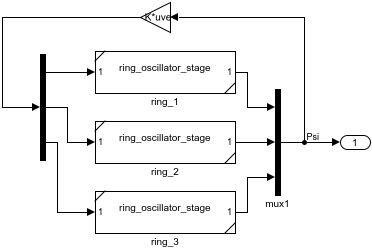
\includegraphics[width=0.7\linewidth]{fig/sim_model_HW6_pblm3}
	\caption{Simulink Model of the feedback system composed of individual nonlinear subsystems}
	\label{fig:simmodelhw6pblm3}
\end{figure}

\begin{figure}[p]
	\centering
	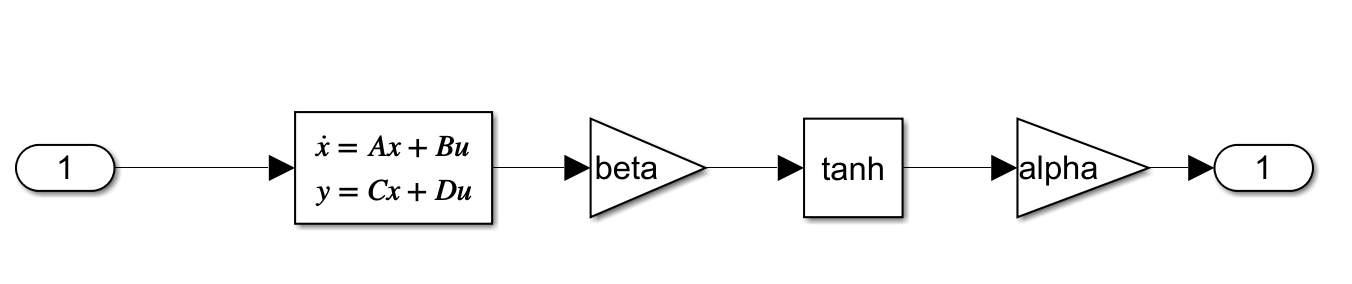
\includegraphics[width=0.7\linewidth]{fig/sim_model_HW6_pblm3_subsystem}
	\caption{Simulink Model of an individual nonlinear subsystem}
	\label{fig:simmodelhw6pblm3subsystem}
\end{figure}


The results for various values of $\mu$ can be seen in \figurename \  \ref{fig:pblm3_mu1}, \figurename \ \ref{fig:pblm3_mu15}, \figurename \ \ref{fig:pblm3_mu2}, \figurename \ \ref{fig:pblm3_mu3}, and \figurename \ \ref{fig:pblm3_mu5}. It is apparent that Asymptotic stability is lost and a limit cycle is gained, in other words, a super-critical hopf-bifurcation occurs. The limit cycle appears to maintain a similar frequency, but as $\mu$ grows (which really means $\beta$ increases based on my code) the magnitude of the limit cycle seems to grow. When it reaches a point where the theoretical magnitude is above the initial conditions it is then truncated (i.e. clipping occurs).


\begin{figure}[p]
	\centering
	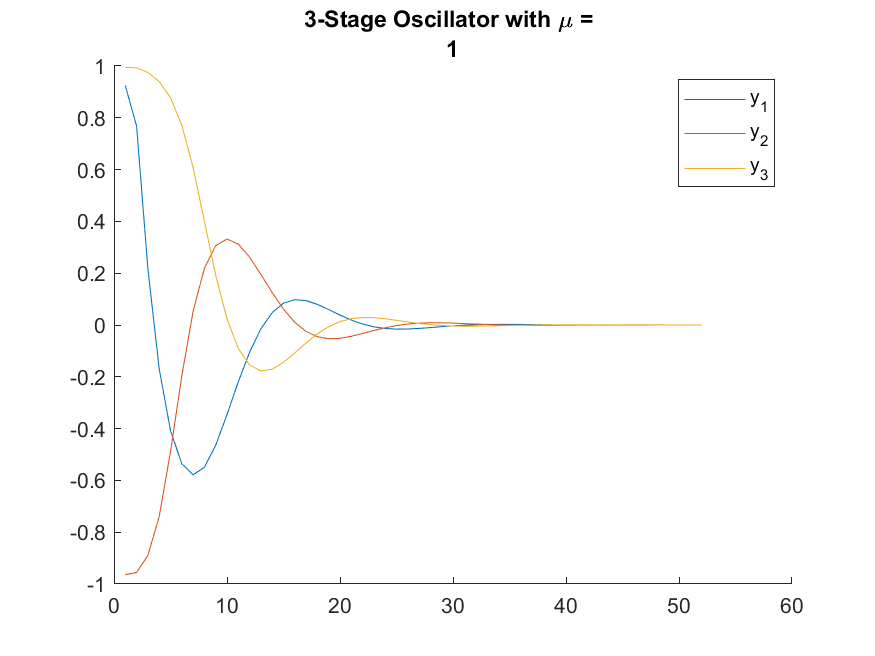
\includegraphics[width=0.7\linewidth]{fig/HW6_pblm3_results_mu_1}
	\caption{Results for the outputs of the 3-stage ring oscillator with mu = 1}
	\label{fig:pblm3_mu1}
\end{figure}

\begin{figure}[p]
	\centering
	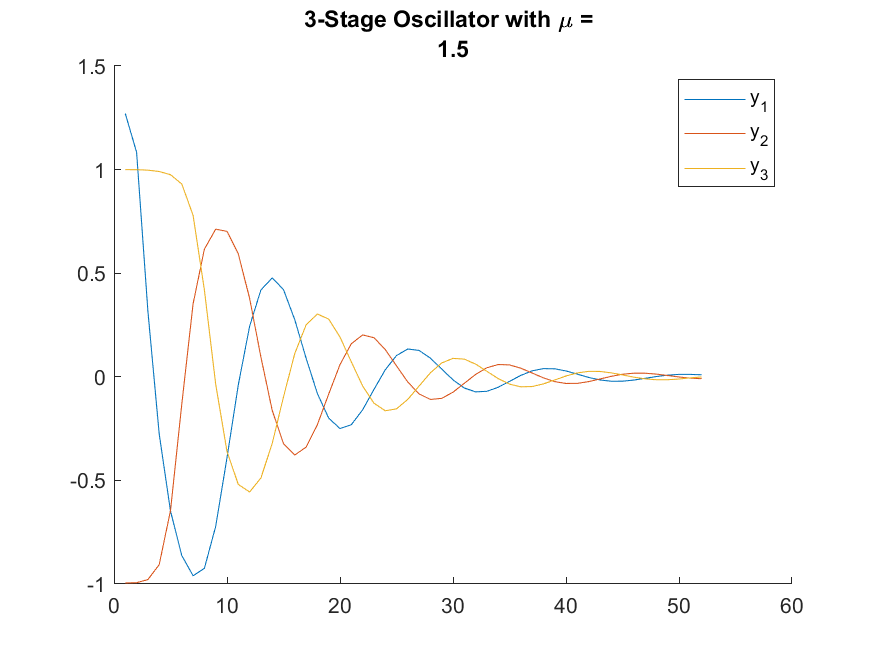
\includegraphics[width=0.7\linewidth]{fig/HW6_pblm3_results_mu_1.5}
	\caption{Results for the outputs of the 3-stage ring oscillator with mu = 1.5}
	\label{fig:pblm3_mu15}
\end{figure}

\begin{figure}[p]
	\centering
	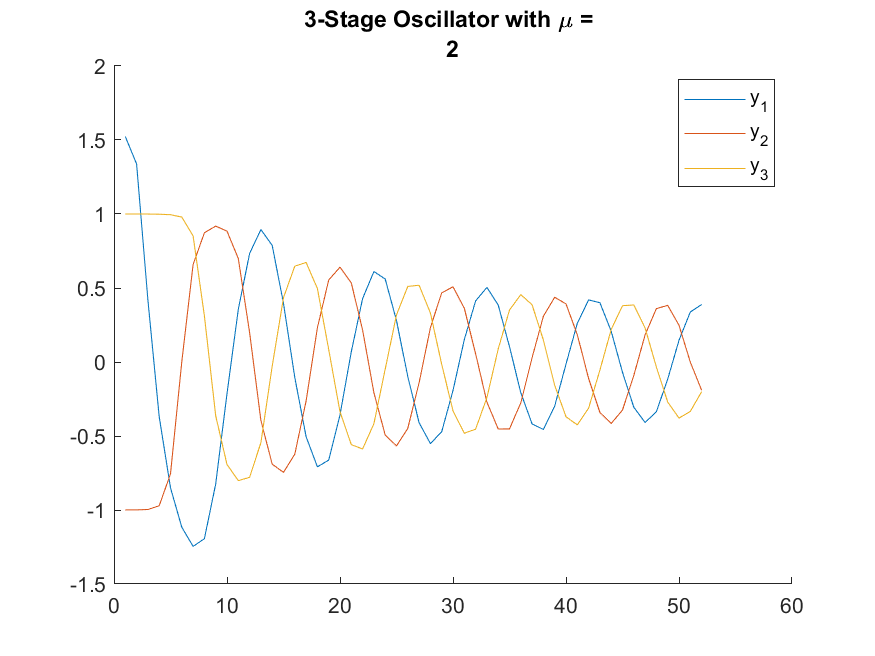
\includegraphics[width=0.7\linewidth]{fig/HW6_pblm3_results_mu_2}
	\caption{Results for the outputs of the 3-stage ring oscillator with mu = 2}
	\label{fig:pblm3_mu2}
\end{figure}

\begin{figure}[p]
	\centering
	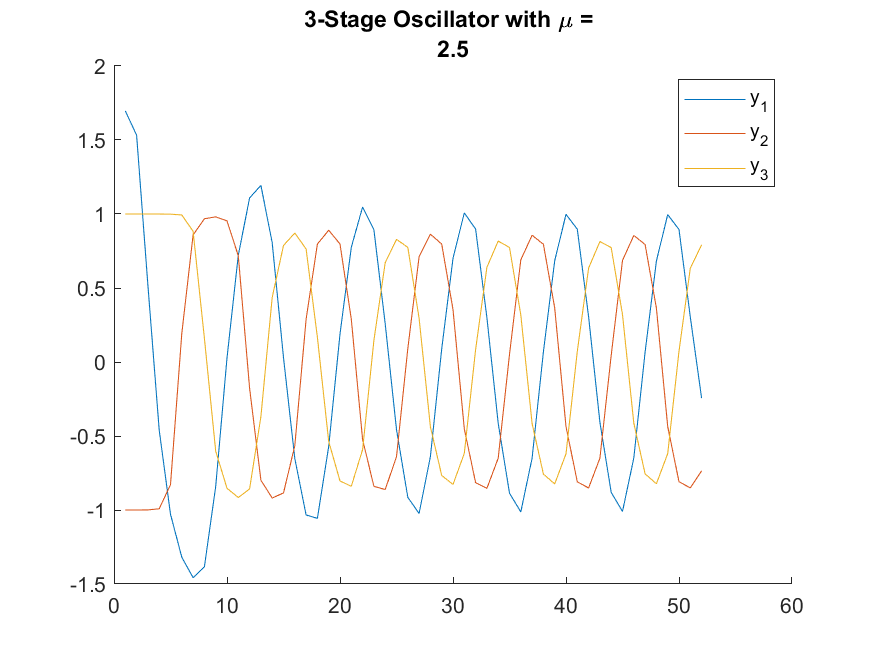
\includegraphics[width=0.7\linewidth]{fig/HW6_pblm3_results_mu_2.5}
	\caption{Results for the outputs of the 3-stage ring oscillator with mu = 2.5}
	\label{fig:pblm3_mu25}
\end{figure}

\begin{figure}[p]
	\centering
	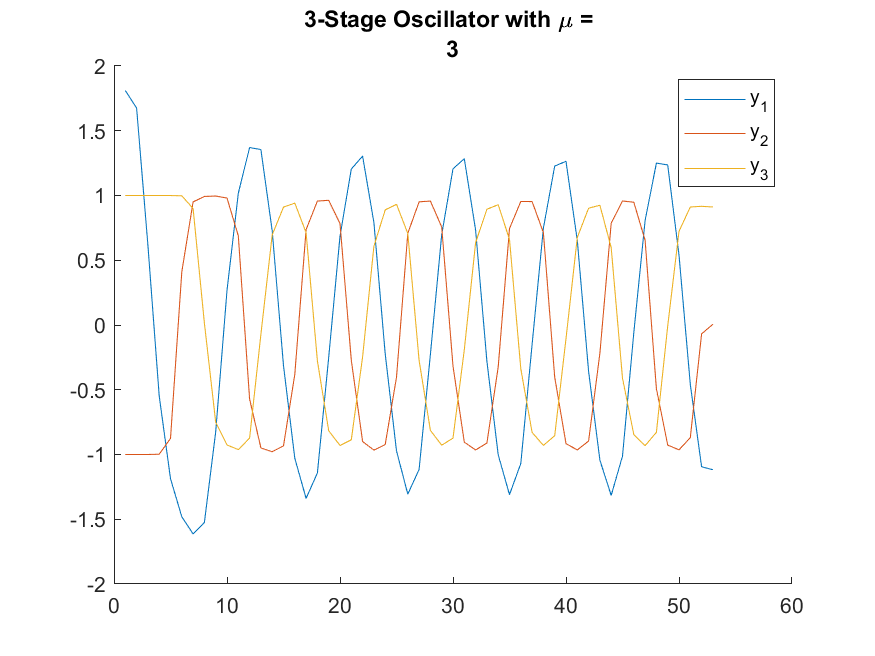
\includegraphics[width=0.7\linewidth]{fig/HW6_pblm3_results_mu_3}
	\caption{Results for the outputs of the 3-stage ring oscillator with mu = 3}
	\label{fig:pblm3_mu3}
\end{figure}

\begin{figure}[p]
	\centering
	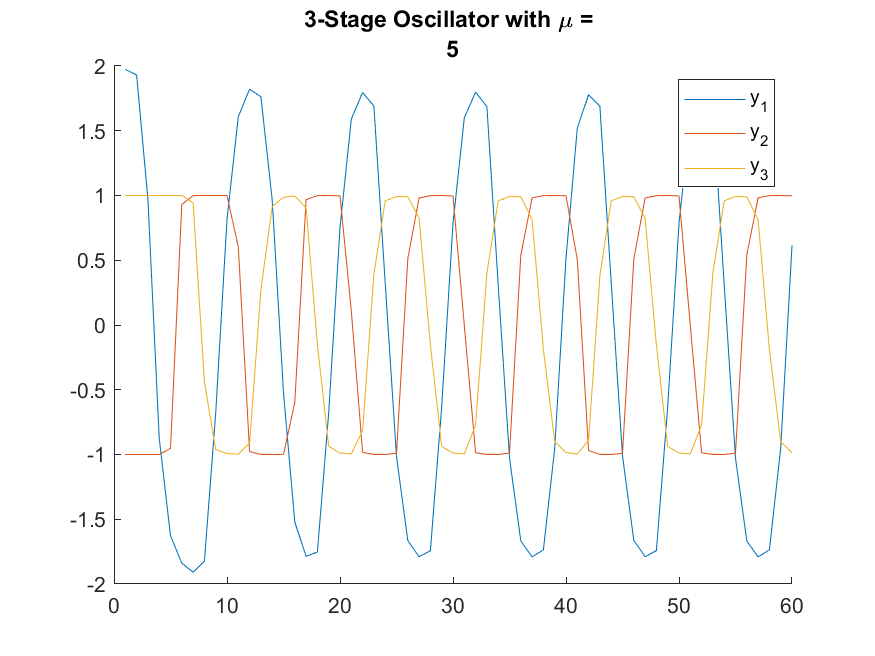
\includegraphics[width=0.7\linewidth]{fig/HW6_pblm3_results_mu_5}
	\caption{Results for the outputs of the 3-stage ring oscillator with mu = 5}
	\label{fig:pblm3_mu5}
\end{figure}




\newpage
\newpage
\newpage
\section{Problem 4}
Consider a set of systems, $H_i (i=1,\dots,n)$, who are coupled together in a feedback given by
$$\mqty[u_1\\ \vdots \\ u_n] = K \mqty[y_1\\ \vdots \\ y_n]$$
for inputs $u_i$ and outputs $y_i$, with feedback matrix $K \in \real^{n\cross n}$.

\begin{figure}[h]
	\centering
	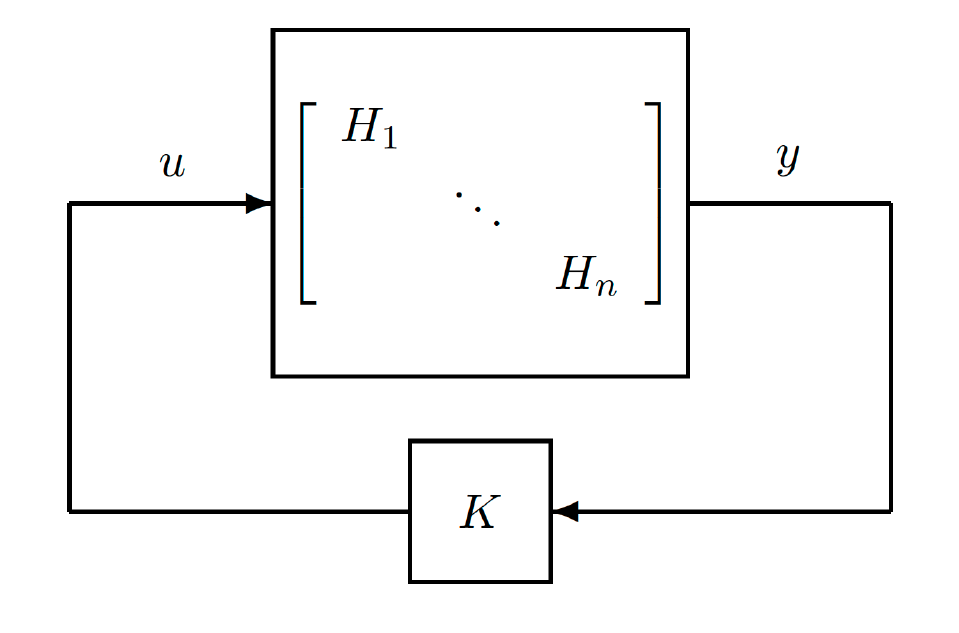
\includegraphics[width=0.5\linewidth]{fig/pblm4_given_fig}
	\label{fig:pblm4givenfig}
\end{figure}

\subsection{Part a (Extra note)}
Suppose each $H_i$ satisfies the dissipation inequality:
$$\dot{V}_i(x_i) \leq -y_i^2 + \gamma_i^2 u_i^2$$
for a Positive Definite function,$V_i(x_i)$, of $x_i$.\\

\newpage
\subsection{Part b}
\textbf{Problem:}
Determine a matrix inequality that restrict the matrices
$$D := \mqty[\dmat{d_1}{\ddots}{d_n}], \ \Gamma := \mqty[\dmat{\gamma_1}{\ddots}{\gamma_n}]$$
and $K$, such that $$V(x) = \sum_{i=1}^{n} d_i V_i(x_i)$$ is a Lyapunov function for the interconnected system.\\

\noindent
\textbf{Solution:}
The stability of a an interconnected system, by definition of the Lyapunov Function, can be proven by ensuring the that $\dot{V}(x)$ is negative definite.

First, Let
\begin{align}
	\dot{V} &= \sum_{i=1}^n d_i V_i, \ d_i \geq 0\\
	&\leq \sum_{i=1}^n d_i \qty(-y_i^2 + \gamma_i^2 u_i^2)\\
	&\leq \sum_{i=1}^n -d_i y_i^2 + d_i \gamma_i^2 u_i^2
	\intertext{which can be put into a Matrix form as}
	\dot{V} &\leq y^T (-D) y + u^T \Gamma^T D \Gamma u
	\intertext{and since $u = Ky$, this becomes}
	\dot{V} &\leq y^T(-D)y + y^T K^T \Gamma^T D \Gamma K y\\
	&\leq y^T \qty(-D + K^T \Gamma^T D \Gamma K) y
\end{align}
Since this exists as an upper bound on $\dot{V}$, the following inequalities are sufficent to say $\dot{V} < 0$ (aka stable)
\begin{align}
	-D + K^T \Gamma^T D \Gamma K &< 0
	\intertext{since D is a diagonal matrix (and thus communtable with other matrices), this can be further reformulated}
	D \qty(- I + K^T \Gamma^T \Gamma K) &< 0
\end{align}
which is equivalent to\footnote{This probably wasn't necessary and lead to the more difficult solution on the next page...}
\begin{align}
	\frac{1}{2} \qty{\qty(- I + K^T \Gamma^T \Gamma K)^T D + D\qty(- I + K^T \Gamma^T \Gamma K)} &< 0
	\intertext{or}
	\qty(- I + K^T \Gamma^T \Gamma K)^T D + D\qty(- I + K^T \Gamma^T \Gamma K) &< 0
\end{align}
which can be used to test the feasibility and find the elements of $D$ to ensure stability.

\subsection{Part c}
\textbf{Problem:}
Investigate when $\exists \ D$ s.t. the inequality is satisfied for $$K = \mqty[0&1\\1&0]$$

\noindent
\textbf{Solution:}
The inequality from the previous problem can be used to asses what conditions must be met for $D$ to exist.
Let, $$D = \mqty[\dmat{d_1}{d_2}]$$ and $$\Gamma = \mqty[\dmat{\gamma_1}{\gamma_2}]$$
These $n=2$ matrices can then be plugged into the inequality as follows
\begin{align}
	\qty(- I + K^T \Gamma^T \Gamma K)^T D + D\qty(- I + K^T \Gamma^T \Gamma K) &< 0
\end{align}
\begin{align}
	\qty(- \mqty[\dmat{1}{1}] + \mqty[0&1\\1&0]^T \mqty[\dmat{\gamma_1}{\gamma_2}]^T \mqty[\dmat{\gamma_1}{\gamma_2}] \mqty[0&1\\1&0])^T \mqty[\dmat{d_1}{d_2}]\hspace{0.25in}\nonumber\\ + \mqty[\dmat{d_1}{d_2}]\qty(- \mqty[\dmat{1}{1}] + \mqty[0&1\\1&0]^T \mqty[\dmat{\gamma_1}{\gamma_2}]^T \mqty[\dmat{\gamma_1}{\gamma_2}] \mqty[0&1\\1&0]) &< 0
\end{align}
\begin{align}
	\qty(-\mqty[\dmat{1}] + \mqty[\dmat{\gamma_1^2}{\gamma_2^2}])^T\mqty[\dmat{d_1}{d_2}] + \mqty[\dmat{d_1}{d_2}]\qty(-\mqty[\dmat{1}{1}] + \mqty[\dmat{\gamma_1^2}{\gamma_2^2}]) &<0\\
	\mqty[\dmat{\gamma_1^2-1}{\gamma_2^2-1}]^T \mqty[\dmat{d_1}{d_2}] + \mqty[\dmat{d_1}{d_2}] \mqty[\dmat{\gamma_1^2-1}{\gamma_2^2-1}] &<0
\end{align}
which (due to communicability of diagonal matrices) can be rewritten as
\begin{align}
	2 \mqty[\dmat{d_1(\gamma_1^2-1)}{d_2(\gamma_2^2-1)}] &< 0
\end{align}
or by analyzing the diagonal values themselves, we have
\begin{align}
	\begin{cases}
		d_1(\gamma_1^2 - 1) < 0\\
		d_2(\gamma_2^2 - 1) < 0
	\end{cases}
\end{align}
in other word, $d_1$ and $d_2$ (and therefore $D$) is possible iff $$\gamma_1^2 < 1 \text{ and } \gamma_2^2 < 1$$

\newpage
\appendix
\section{MATLAB Code:}\label{apx:matlab}
All code I write in this course can be found on my GitHub repository:\\
\href{https://github.com/jonaswagner2826/MECH6313}{https://github.com/jonaswagner2826/MECH6313}
% MECH6313_HW6
\lstinputlisting[caption={MECH6313\_HW6},label={script:HW6}]{MECH6313_HW6.m}

\newpage
\section{MATLAB Code for Problem 3:}\label{apx:matlabpblm3}
% MECH6313_HW6_pblm3
\lstinputlisting[caption={MECH6313\_HW6\_pblm3},label={script:HW6_pblm3}]{MECH6313_HW6_pblm3.m}


\end{document}
